% METODOLOGIA------------------------------------------------------------------

\chapter{Metodologia}
\label{chap:metodologia}

% LEMBRAR DE NÃO FALAR DO SILVIO AQUI

A metodologia empregada neste trabalho está organizada nos seguintes passos principais:

\begin{description}
\item[Etapa 1] Aquisição da base de vídeos UCF50 - Action Recognition Data Set \citeauthor{reddy2013recognizing}.
\item[Etapa 2] Aplicação das 14 distorções descritas na Seção~\ref{sec:ataques} sobre a base.
\item[Etapa 3] Geração das assinaturas utilizando os algoritmos baseados em diferença de quadro, gradientes, medida ordinal, quadros de cena, padrão binário por região e wavelets, descritos no Capítulo~\ref{chap:revisao}.
\item[Etapa 4] Realização do procedimento de comparação de um conjunto de treinamento das assinaturas, a fim de definir um limiar para classificação.
\item[Etapa 5] Realização do procedimento de comparação de um conjunto de testes das assinaturas, a partir dos limiares obtidos na Etapa 4.
\item[Etapa 5] Análise comparativa dos resultados obtidos a partir da Etapa 4. Os resultados desta etapa serão discutidos em detalhes no próximo capítulo.
\end{description}

As seções a seguir detalham como esses passos serão realizados.

\section{Definição e Obtenção da Base de Vídeos}
\label{sec:database}

Para a realização dos experimentos desta monografia, foi escolhida a base de vídeos UCF50 - Action Recognition Data Set \citeauthor{reddy2013recognizing}, que é comumente utilizada em projetos de reconhecimento de movimento humano. Ela foi escolhida pela quantidade de vídeos que contém, além de sua licença de livre utilização.

Ela está segmentada em 50 categorias diferentes que representam ações do quotidiano, como por exemplo ciclismo, natação, caminhada com o cachorro, TaiChi, etc. Dentro de cada categoria, há pelo menos 4 vídeos pertencentes a uma mesma gravação, apresentando assim os mesmos personagens, fundo e ponto de vista. A fim de reduzir o número de vídeos que apresentam o mesmo conteúdo, foram selecionados apenas o primeiro vídeo de cada grupo.

A base original é composta de 6.681 vídeos com duração média entre 3 a 9 segundos e após a seleção descrita no parágrafo anterior, restaram 1.264 vídeos. Para cada vídeo selecionado foram aplicadas as distorções descritas na Seção~\ref{sec:ataques}, totalizando 18.960 itens, sendo destes, 17.696 vídeos resultantes das distorções. A Figura~\ref{fig:exemplos} apresenta alguns exemplos de vídeos da base.

\begin{figure}
    \centering
    \caption{Exemplos de vídeos retirados da base. O primeiro mostra um jogo de baseball, o segundo mostra uma criança fazendo malabarismo, o terceiro mostra uma competição de levantamento de pesos}
    \label{fig:exemplos}
    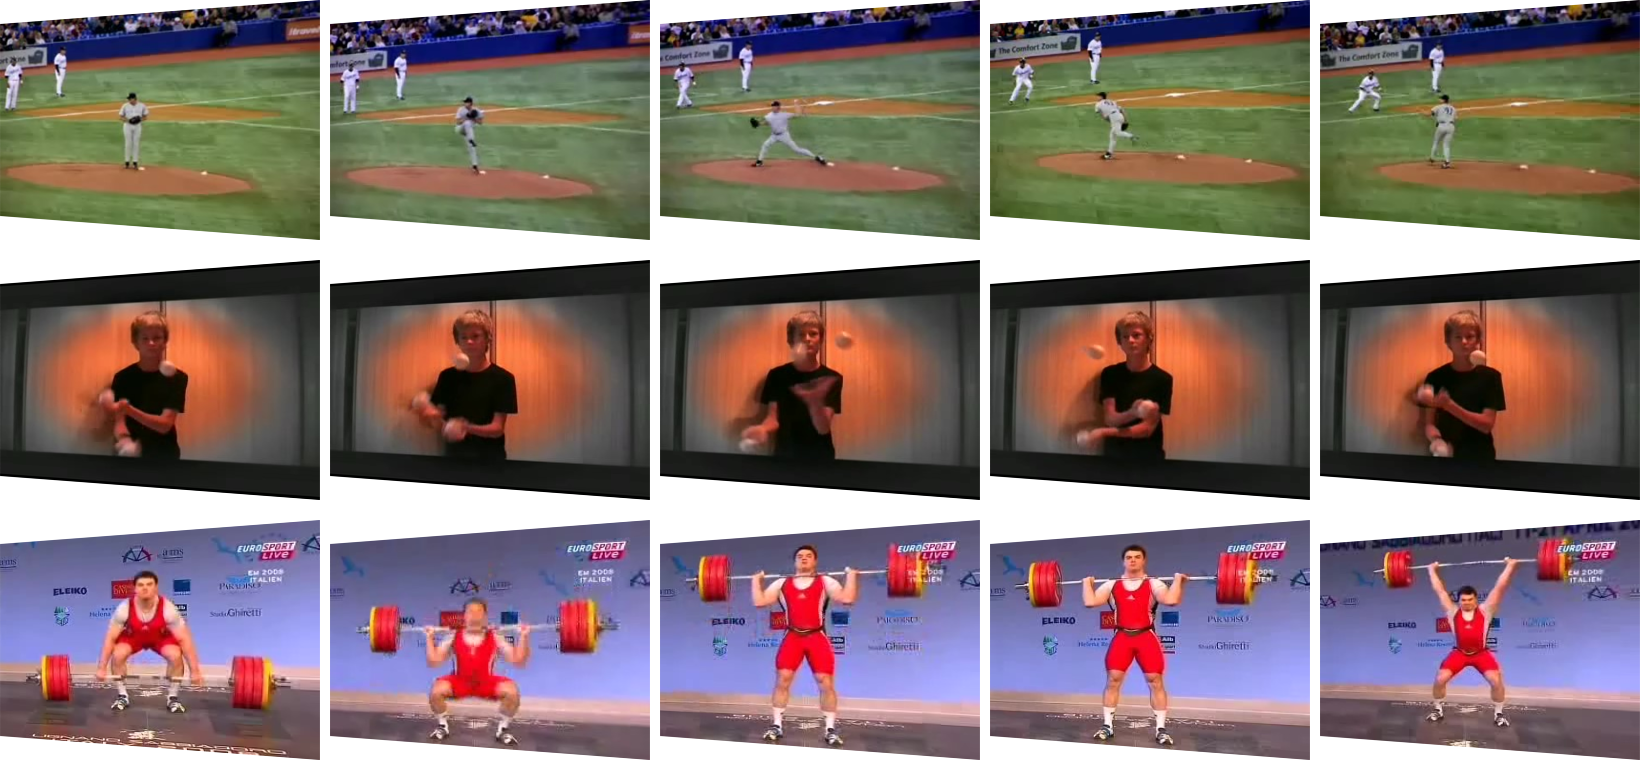
\includegraphics[width=0.8\textwidth]{dados/figuras/exemplos.png}
\end{figure}

\section{Aplicação das Distorções}
\label{sec:met-distorcoes}

Para a criação de um conjunto de cenários de treinamento e teste, foram aplicadas as 14 distorções descritas na Seção~\ref{sec:ataques} sobre os 1.264 vídeos selecionados da base UCF50, totalizando 17.696 vídeos distorcidos. Estes cenários propiciam a avaliação do desempenho das diferentes assinaturas revisadas neste trabalho quanto à robustez e a unicidade quando os vídeos são submetidos a diferentes tipos de distorções. A fim de garantir a reprodutibilidade do experimento, os parâmetros utilizados para a aplicação de cada uma das distorções são explicitados na Tabela~\ref{tab:params}. Para facilitar a discussão dos resultados, serão utilizadas as siglas definidas na primeira coluna da tabela quando houve referência às distorções.

\begin{table}[h]
\centering
\caption{Parâmetros usados na aplicação das distorções}
\label{tab:params}
\begin{tabular}{|p{0.2\textwidth}|p{0.4\textwidth}|p{0.4\textwidth}|} \hline
    \textbf{Sigla} & \textbf{Distorção} & \textbf{Parâmetros} \\ \hline
    TEXT & Adição de texto e legendas & \\ \hline
    WATERMARK & Adição de Marca D'água & \begin{tabular}{@{}l@{}}Texto: "Copyright"\\ Tamanho da fonte: 20\\ Opacidade: 65\% \end{tabular}\\ \hline
    BORDER & Adição de Quadro ou Bordas & Tamanho da borda: 25 pixels \\ \hline
    BIG & Redimensionamento da Altura e Largura dos Vídeos para Maior & \begin{tabular}{@{}l@{}} Fator de redimensionamento: 2\\ MANTÉM aspect ratio: sim \end{tabular} \\ \hline
    CROP & Eliminação de uma faixa ou região dos quadros &  \\ \hline
    FLOP & Inversão/espelhamento & Sentido: horizontal \\ \hline
    ROTATE & Rotação & 10 graus \\ \hline
    BLUR & Desfoque & \begin{tabular}{@{}l@{}}Tipo: gaussiano\\ Sigma: 3\end{tabular} \\ \hline
    COLOR & Inversão das cores &  \\ \hline
    JPEG & Alteração das compressão dos quadros do vídeo & Compressão utilizada: JPEG \\ \hline
    FAST1 & Aceleração do vídeo 1 & Aumento da velocidade em 50\% \\ \hline
    FAST2 & Aceleração do vídeo 2 & Aumento da velocidade em 25\% \\ \hline
\end{tabular}
\end{table}

\section{Geração das Assinaturas}
\label{sec:met-assinaturas}

O passo final de preparação para os experimentos deste trabalho foi a criação das assinaturas utilizando os 6 algoritmos descritos no Capítulo~\ref{chap:revisao}. As assinaturas foram geradas para todos os 17.696 vídeos originais e distorcidos, totalizando 106.176 assinaturas. Para facilitar a consulta dos resultados do experimento, todas as assinaturas foram arquivadas em um banco de dados contendo dados do vídeo a qual a assinatura pertence, se o vídeo é um vídeo original ou um distorcido, o tipo da distorção e uma referência ao vídeo original, além do tipo de assinatura utilizado. A Tabela~\ref{tab:assinaturas} apresenta todas as assinaturas sendo utilizadas, junto do intervalo numérico em que as assinaturas se encontram, além dos tipos de características de um vídeo utilizados para obtê-las. A primeira coluna da tabela apresenta a sigla de cada assinatura que será utilizada na Seção de Resultados.

\begin{table}[h]
    \centering
    \caption{Assinaturas utilizadas para comparação}
    \label{tab:assinaturas}
    \begin{tabular}{|p{0.2\textwidth}|p{0.259\textwidth}|p{0.259\textwidth}|p{0.259\textwidth}|} \hline
        \textbf{Sigla} & \textbf{Assinatura} & \textbf{Características} & \textbf{Intervalo de Dados} \\ \hline
        gradient & Gradiente & - & [0-1] \\ \hline
        framedif & FrameDiff & - & [0-1] \\ \hline
        medidaordina & Medida Ordinal & - & [0-1] \\ \hline
        wavelet & Wavelets & - & [0-1] \\ \hline
        rb & RBP & - & [0-1] \\ \hline
        scenefram & Scene Frame & - & [0-1] \\ \hline
    \end{tabular}
\end{table}

\section{Comparação de Assinaturas}
\label{sec:met-comparacao}

As assinaturas geradas na etapa anterior são compostas de vetores de características e cada um dos algoritmos geradores descreve uma forma de compará-los, geralmente utilizando a distância euclidiana ou a distância de manhattan. Para simplificar a implementação e análise dos resultados, foi necessária a escolha de uma medida única capaz de lidar com as características de cada assinatura. Um dos fatores a ser considerado é que o tamanho das assinaturas é proporcional ao tamanho dos vídeos dos quais elas provém, além disso, este trabalho usa algumas distorções do tipo temporal que alteram a velocidade e o \textit{framerate} de vídeos, alterando seu tamanho. Sendo assim, a medida utilizada precisa lidar com assinaturas de tamanhos e frequências diferentes.

Enquanto a distância Euclidiana pode ser útil para comparar as assinaturas de um único quadro de cada vídeo, o fato dela comparar cada valor de duas assinaturas de um em um a torna suscetível a distorções temporais. Para resolver os problemas mencionados, foi escolhido o DTW (\textit{Dynamic Time Warping}) como forma de comparação, uma técnica conhecida para alinhamento entre duas sequências temporais. Originalmente, esta técnica foi utilizada para a comparação de diferentes padrões vocais em aplicações de reconhecimento de voz, mas o DTW já foi utilizado com sucesso para lidar com deformações temporais e velocidades diferentes em dados dependentes de tempo, explica \citeauthor{muller2007dynamic}. A Figura~\ref{fig:dist-comparacao} mostra um comparativo entre o funcionamento da distância Euclidiana e do DTW, nota-se o pareamento $1:1$ da distância Euclidiana (imagem de cima), e o pareamento $n:1$ do DTW.

\begin{figure}[h]
    \centering
    \caption{Distância entre duas sequências temporais medida usando distância euclidiana (na imagem de cima) e o DTW (na imagem de baixo)}
    \label{fig:dist-comparacao}
    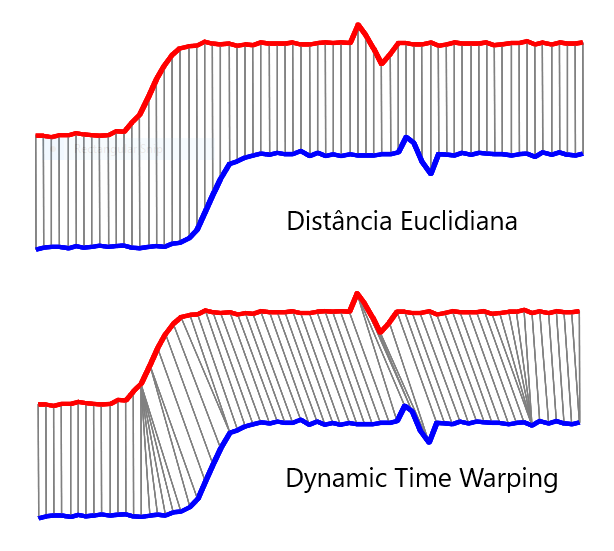
\includegraphics[width=0.6\textwidth]{dados/figuras/dtw-euclidiana.png}
\end{figure}

Para achar esse pareamento, o DTW compara todos os valores das duas sequências do início ao fim utilizando uma medida de distância (normalmente distância de Manhattan ou Euclidiana) e o valor mínimo das 3 comparações anteriores, o resultado é uma matriz de custo, como mostra a Figura~\ref{fig:dtw-caminho}. Em seguida, percorre-se a matriz da última célula até a primeira, sempre escolhendo a célula com o menor custo como próximo passo. O caminho formado é o pareamento entre valores das duas sequências temporais.


\begin{figure}[h]
    \centering
    \caption{a) Matriz de custo formada comparando duas sequências temporais. b) Caminho com menor custo}
    \label{fig:dtw-caminho}
    \begin{tabular}{ll}
    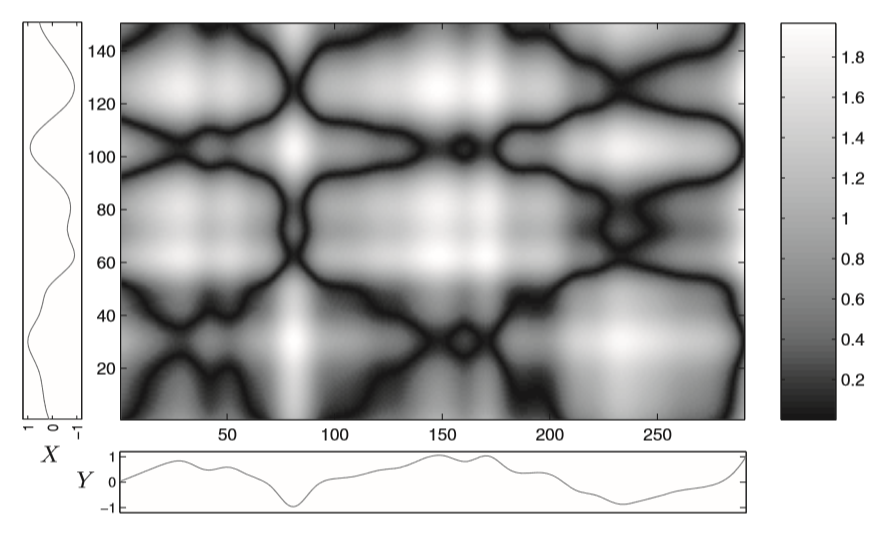
\includegraphics[width=0.4\textwidth]{dados/figuras/dtw-comparacao.png} &
    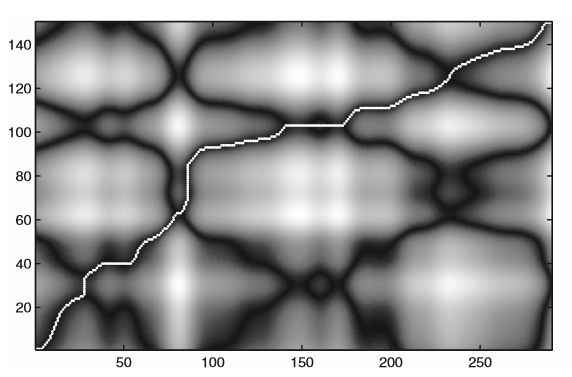
\includegraphics[width=0.4\textwidth]{dados/figuras/dtw-comparacao-caminho.png} \\
    a) Matriz de custo & b) Caminho mais barato
    \end{tabular}
\end{figure}

% Fórmula do DTW

Em sua forma original, o DTW tem uma complexidade de $ O(N^{2}) $, por este motivo, foi utilizada uma variante do algoritmo chamada FastDTW, que provém alinhamentos ótimos ou quase ótimos com complexidade de $O(N)$.

% falar que precisa normalizar

\section{Experimentos}
\label{sec:met-Experimentos}

% divisão entre treinamento, validação e teste

\section{Análise dos Resultados}
\label{sec:met-analise}


% Foi escolhida a linguagem Python (versão 2.7.12) para a implementação dos algoritmos por ser multiplataforma e  por sua simplicidade na integração com bibliotecas de alta-performance implementadas em linguagens de baixo nível (C). Isto foi importante pois serão utilizadas as bibliotecas \textit{OpenCV} (versão 3.0.0) e \textit{NumPy} (versão 1.12.1) para manipulação e operação de imagens.

% Para a compilação da base de vídeos foi utilizada a biblioteca MagicImage (versão 7.0.7-8-Q16-x64 - Windows), que incluí os programas \textit{convert} e \textit{ffmpeg}, utilizados para conversão de formatos, aplicação de distorções e transformações de vídeo e imagem respectivamente.

% \section{Definição e Implementação do método de comparação}


% \textbf{[EM DESENVOLVIMENTO]}

% pegar base de assinaturas distrocidas, e para cada distorçao, calcular a distancia para todas as assinaturas originais

% pegar as duas menores distancias para cada distorçao de cada vídeo

% se a dif do primeiro colocado (primera distancia) for diferente o suficiente para o segundo colocado , entao podemos assumir (podemos?) que encontramos a assinatura do vídeo original

% EMBASAR ESSAS PARADAS LOUCAS

% \section{Validação das implementações}

% Antes de realizar-se qualquer experimento, é necessário que os algoritmos implementados passem por uma etapa de validação que consiste em comparar seus resultados com os dos artigos de base. Para isso serão revisados os artigos dos quais os algoritmos foram retirados, além de códigos disponibilizados através destes trabalhos.

% A validação ocorrerá em duas etapas:

% \begin{enumerate}
% \item teste de software;
% \item comparação das saídas dos algoritmos implementados para o trabalho e as implementações originais, dada a mesma entrada.
% \end{enumerate}

% \section{Definição dos Experimentos}
% \label{sec:definicaoexperimentos}